\documentclass[12pt]{article}

\usepackage[vmargin=1in,hmargin=1in]{geometry}
\usepackage{amsmath}
\usepackage[parfill]{parskip}
\usepackage{hyperref}
\usepackage{natbib}
\usepackage{bm}
\usepackage{amsfonts}
\usepackage{graphicx}
\usepackage{abstract}
\usepackage{lineno}
\usepackage{setspace}

\hypersetup{pdfstartview={Fit},hidelinks}


\usepackage{caption}
\captionsetup[figure]{labelformat=empty}% redefines the caption setup of the figures environment in the beamer class.


\title{Ecological Applications Appendix S1 \\ Simulation study accompanying the paper: \\ \it Monitoring partially-marked populations using camera and telemetry data }
\author{Lydia L. S. Margenau$^{1}$\footnote{Corresponding author: lydia.margenau@wisconsin.gov}, Michael J. Cherry$^2$,  Karl V. Miller$^1$, \\ Elina P. Garrison$^3$, Richard B. Chandler$^1$}


\begin{document}



\maketitle

\vspace{12pt}

\begin{description}%[labelindent=1pt]%[leftmargin=1cm]%,labelwidth=\widthof{\bfseries Example:}]
%  \large
\item[$^1$] Warnell School of Forestry and Natural Resources, University of Georgia %\\
\item[$^2$] Caesar Kleberg Wildlife Research Institute at Texas A\&M University-Kingsville %\\
\item[$^3$] Florida Fish and Wildlife Conservation Commission %\\
\end{description}

\clearpage

\section*{Introduction and Methods}

We conducted a small simulation study to compare the performance of
the joint generalized spatial mark-resight (gSMR) model with the
two-stage gSMR model. One hundred datasets were simulated from the
model with parameters chosen to resemble the deer study described in
the manuscript. Specifically, parameters were $\beta_0=1$,
$\beta_1=-0.02$, $\alpha=0.5$, $\sigma_{\epsilon}=0.1$,
$\lambda_0=0.07$, and $\sigma=400$. For the joint model, we assumed a
uniform marking process with $p^{\rm cap}=0.2$. The design involved 60
cameras with the same spatial arrangement as the cameras at our AL
study site. We modeled the population over 20 primary sampling
periods, each corresponding to a 14-day period. We simulated one
telemetry location per day. Code to reproduce the simulation study can
be found at \url{https://github.com/rbchan/monitor-cam-telem}.


\section*{Results and Discussion}

The number of individuals captured and outfitted with telemetry
devices ranged from 13--35 in the simulated datasets. As with the deer
example, only a small fraction (ranging from 0--10) were detected by
cameras. 



\clearpage

\begin{figure}[h!]
  \centering
  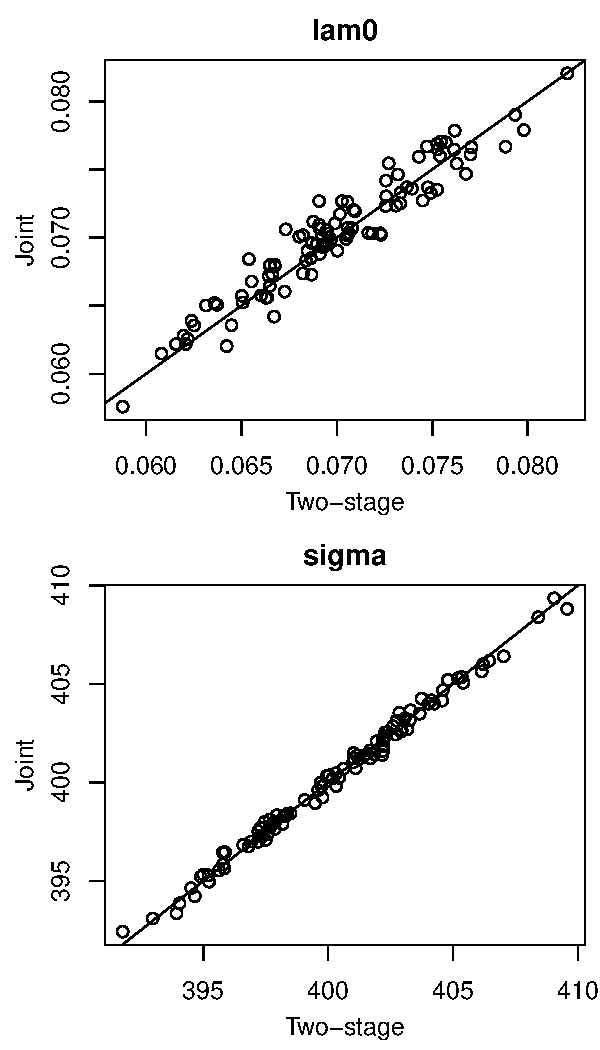
\includegraphics[width=0.7\textwidth]{sim/sim-lam0sig}
  \caption{Figure S1. Results from the 100 simulated datasets used to
    compare posterior means for the encounter rate parameters
    ($\lambda_0$ and $\sigma$) for the joint model and the two-stage
    model. }   
  \label{fig:sim-lam0sig}
\end{figure}


\clearpage

\begin{figure}[h!]
  \centering
  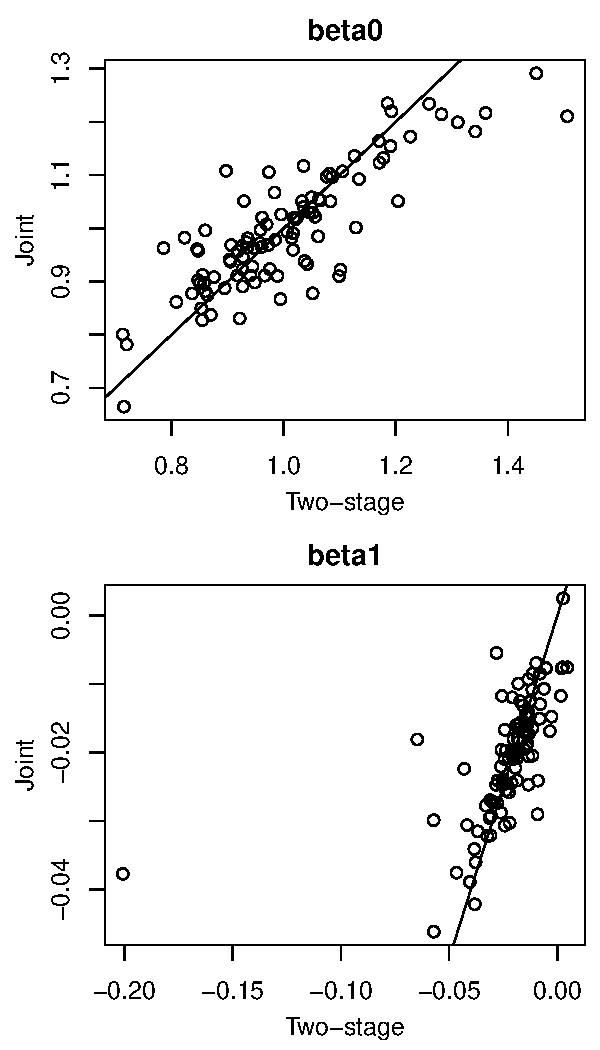
\includegraphics[width=0.7\textwidth]{sim/sim-betas}
  \caption{Figure S1. Results from the 100 simulated datasets used to
    compare posterior means for the density trend parameters
    ($\beta_0$ and $\beta_1$) for the joint model and 
    the two-stage model. }  
  \label{fig:sim-betas}
\end{figure}



\end{document}


